\chapter{Main Window}

The only fixed UI elements in ngscopeclient are the main menu and toolbar at the top of the window. All remaining space
may be filled with waveform plots, properties dialogs, protocol analyzers, and other dockable windows as required for a
given experimental setup. This flexibility allows almost the entire screen to be dedicated to waveform views, or more
space allocated to controls and protocol decodes.

\section{Menu}

%%%%%%%%%%%%%%%%%%%%%%%%%%%%%%%%%%%%%%%%%%%%%%%%%%%%%%%%%%%%%%%%%%%%%%%%%%%%%%%%%%%%%%%%%%%%%%%%%%%%%%%%%%%%%%%%%%%%%%%%
\subsection{File}

This menu contains commands for saving and loading session files.

\begin{itemize}

\item \menustyle{Open Online...}\\
Loads a session file and reconnects to the instrument(s) to continue existing work. Settings from the saved
session will be applied and overwrite the current channel and timebase configuration of the instrument, if different.

\item \menustyle{Open Offline...}\\
Loads a session file in offline mode, allowing you to work with saved waveform data without connecting to the
instrument(s) the data was captured from.

\item \menustyle{Recent Files}\\
Displays a list of recently accessed session files and allows them to be opened online or offline.

\item \menustyle{Save}\\
Saves UI configuration and waveform data (including history) to a session file for future use.

A session consists of a YAML file called \emph{filename}.scopesession containing instrument and UI configuration, as
well as a directory called \emph{filename}\_data which contains waveform metadata and sample values for all enabled
instrument channels, including history.

Note that both the .scopesession and the \_data directory must be copied if moving the session to a new location in
order to preserve waveform data. If you only wish to restore the filter graph and UI configuration without waveform
content, the \_data directory is not required.

\item \menustyle{Save As...}\\
Saves the session to a new file, rather than the current one.

\item \menustyle{Close}\\
Close the current session without exiting ngscopeclient.

\item \menustyle{Quit}\\
Exits the application

\end{itemize}

%%%%%%%%%%%%%%%%%%%%%%%%%%%%%%%%%%%%%%%%%%%%%%%%%%%%%%%%%%%%%%%%%%%%%%%%%%%%%%%%%%%%%%%%%%%%%%%%%%%%%%%%%%%%%%%%%%%%%%%%
\subsection{View}

\begin{itemize}

\item \menustyle{Fullscreen}\\
Toggles full-screen mode

\item \menustyle{Persistence Setup}\\
Opens the Persistence Setup dialog, allowing you to control the decay coefficient for persistence maps.

\end{itemize}

%%%%%%%%%%%%%%%%%%%%%%%%%%%%%%%%%%%%%%%%%%%%%%%%%%%%%%%%%%%%%%%%%%%%%%%%%%%%%%%%%%%%%%%%%%%%%%%%%%%%%%%%%%%%%%%%%%%%%%%%
\subsection{Add}

This menu allows new waveforms views or instrument connections to be created.

\begin{itemize}

\item \menustyle{Load}\\
Connect to a new, or recently used, electronic load

\item \menustyle{Generator}\\
Connect to a new, or recently used, function generator

\item \menustyle{Multimeter}\\
Connect to a new, or recently used, multimeter

\item \menustyle{Oscilloscope}\\
Connect to a new, or recently used, oscilloscope

\item \menustyle{Power Supply}\\
Connect to a new, or recently used, power supply

\item \menustyle{RF Generator}\\
Connect to a new, or recently used, RF signal generator

\item \menustyle{Channels}\\
Displays a list of filters and instrument channels which can be opened in a new waveform view

\item \menustyle{Generate}\\
Allows synthetic waveforms to be generated for testing, simulation, and channel design applications

\item \menustyle{Import}\\
Allows waveforms to be loaded from external data files in various interchange formats

\end{itemize}

%%%%%%%%%%%%%%%%%%%%%%%%%%%%%%%%%%%%%%%%%%%%%%%%%%%%%%%%%%%%%%%%%%%%%%%%%%%%%%%%%%%%%%%%%%%%%%%%%%%%%%%%%%%%%%%%%%%%%%%%
\subsection{Setup}

\begin{itemize}

%\item \menustyle{Instrument Sync}\\
%Synchronizes two or more instruments under a single ngscopeclient instance. TODO: more complete documentation

\item \menustyle{Timebase...}\\
Opens the Timebase Properties dialog, allowing sample rate and memory depth of each connected oscilloscope to be
adjusted

\item \menustyle{Trigger...}\\
Configures trigger settings

%\item \menustyle{Halt Conditions}\\
%Makes ngscopeclient pause when a waveform meeting certain conditions is acquired

\item \menustyle{Preferences...}\\
Opens the preferences dialog

\end{itemize}

\begin{comment}

\begin{tabularx}{16cm}{llX}
\thickhline
\textbf{Name} & \textbf{Colors} & \textbf{Notes} \\
\thickhline
CRT & 
\includegraphics[width=5cm]{images/eye-gradient-crt.png} & Similar to a major vendor's color scheme.\\
Grayscale & 
\includegraphics[width=5cm]{images/eye-gradient-grayscale.png} & Common monochrome palette.\\
Ironbow & 
\includegraphics[width=5cm]{images/eye-gradient-ironbow.png} & Common "hot metal" palette. \\
KRain & 
\includegraphics[width=5cm]{images/eye-gradient-krain.png} & Similar to a major vendor's color scheme.\\
Rainbow & 
\includegraphics[width=5cm]{images/eye-gradient-rainbow.png} & Common HSV rainbow palette. \\
Reverse Rainbow & 
\includegraphics[width=5cm]{images/eye-gradient-reverse-rainbow.png} & Common HSV rainbow palette. \\
Viridis & 
\includegraphics[width=5cm]{images/eye-gradient-viridis.png} & Perceptually uniform palette from matplotlib. \\
\thickhline
\end{tabularx}

\end{comment}

%%%%%%%%%%%%%%%%%%%%%%%%%%%%%%%%%%%%%%%%%%%%%%%%%%%%%%%%%%%%%%%%%%%%%%%%%%%%%%%%%%%%%%%%%%%%%%%%%%%%%%%%%%%%%%%%%%%%%%%%
\subsection{Window}

This menu provides access to various utility windows.

\begin{itemize}

\item \menustyle{Analyzer}\\
Opens protocol analyzer dialogs for active protocol decodes

\item \menustyle{Generator}\\
Opens the properties dialog for a currently connected function generator

\item \menustyle{Multimeter}\\
Opens the properties dialog for a currently connected multimeter

\item \menustyle{SCPI Console}\\
Opens a console window allowing you to send raw SCPI commands to a currently connected instrument.

This is a low level debug tool primarily intended for use by driver developers. The console is interlocked with
background threads polling the instrument, so that replies to commands typed in the console will not be mixed with
replies which the instrument driver is expecting to its own commands. However, commands sent in the console will bypass
any caching in the driver and can easily lead to the driver and instrument firmware states becoming mutually
inconsistent.

\item \menustyle{Log Viewer}\\
Opens a console window allowing you to see debug log messages generated by the application. This is the same log stream
which is normally written to stdout, but this dialog allows it to be accessed even when the application is not launched
from a shell session.

\item \menustyle{Measurements}\\
Opens the Measurements window, displaying scalar-valued measurements coming from instrument channels or filter blocks.

\item \menustyle{Performance Metrics}\\

Opens the Performance Metrics window, which provides access to debug information which can be helpful when debugging
slow application performance, optimizing the code, or benchmarking instruments.

Three categories of information are displayed:

\begin{itemize}
\item Rendering: render loop framerate, monitor refresh rate, total time spent last frame in the rasterization and tone
mapping shaders, and the number of vertices and indices drawn as Vulkan geometry. Note that waveforms are drawn by a
compute shader and do not contribute towads the vertex/index totals, other than a single textured rectangle used for
displaying the shader output.
\item Filter graph: number of filter blocks in the current graph, and run time for the most recent evaluation of the
filter graph.
\item Acquisition: streaming data rate, in waveforms per second.
\end{itemize}

\item \menustyle{History}\\

Opens the History dialog, which allows access to a rolling buffer of recently acquired waveforms.

\item \menustyle{Filter Graph}\\
Opens the filter graph editor (see Chapter \ref{grapheditor})

\end{itemize}

%%%%%%%%%%%%%%%%%%%%%%%%%%%%%%%%%%%%%%%%%%%%%%%%%%%%%%%%%%%%%%%%%%%%%%%%%%%%%%%%%%%%%%%%%%%%%%%%%%%%%%%%%%%%%%%%%%%%%%%%

\subsection{Debug}

Provides access to GUI toolkit test dialogs and other features intended only for developers.

%%%%%%%%%%%%%%%%%%%%%%%%%%%%%%%%%%%%%%%%%%%%%%%%%%%%%%%%%%%%%%%%%%%%%%%%%%%%%%%%%%%%%%%%%%%%%%%%%%%%%%%%%%%%%%%%%%%%%%%%

\subsection{Help}

Nothing here yet, we should add at least an About dialog at some point...

%\textbf{About}: Displays program version and copyright information

\begin{comment}
%%%%%%%%%%%%%%%%%%%%%%%%%%%%%%%%%%%%%%%%%%%%%%%%%%%%%%%%%%%%%%%%%%%%%%%%%%%%%%%%%%%%%%%%%%%%%%%%%%%%%%%%%%%%%%%%%%%%%%%%
\section{Toolbar}

The toolbar contains buttons and controls for the most frequently used actions.

\begin{figure}[h]
\centering

\includegraphics[width=16cm]{images/toolbar.png}
\caption{ngscopeclient toolbar}
\label{toolbar}
\end{figure}

\subsection{Capture buttons}

The capture button group (Fig. \ref{capturebuttons}) contains three buttons. From left to right these are ``arm
normal trigger", ``arm one-shot trigger" and ``stop trigger".

Note that the ``normal" trigger mode still uses one-shot capture internally so that all waveform data can be downloaded
before the next trigger event.

\begin{figure}[h]
\centering

\includegraphics[height=1cm]{images/capture-icons.png}
\caption{Capture control buttons}
\label{capturebuttons}
\end{figure}

\subsection{History}

The history button (Fig. \ref{historybutton}) toggles display of the \hyperref[sec:history]{waveform history view}.

\begin{figure}[h]
\centering

\includegraphics[height=1cm]{images/history-button.png}
\caption{History button}
\label{historybutton}
\end{figure}

\subsection{Refresh Settings}

In order to improve performance, ngscopeclient caches many instrument settings locally rather than constantly querying
the instrument for the current timebase, trigger configuration, etc. If settings are changed via the instrument front
panel while ngscopeclient is running, ngscopeclient may not be aware of these changes.

The Refresh Settings button (Fig. \ref{refreshbutton}) clears all cached instrument configuration and updates
ngscopeclient with the current instrument settings. For most ``headless" instruments, such as Pico Technology devices,
this button has no effect.

\begin{figure}[h]
\centering

\includegraphics[height=1cm]{images/refresh-button.png}
\caption{Refresh Settings button}
\label{refreshbutton}
\end{figure}

\subsection{Clear Sweeps}

The Clear Sweeps button (Fig. \ref{clearbutton}) clears all persistence waveforms, accumulated eye pattern / waterfall
data, and statistics. Waveforms saved in history are not deleted.

\begin{figure}[h]
\centering

\includegraphics[height=1cm]{images/clear-button.png}
\caption{Clear Sweeps button}
\label{clearbutton}
\end{figure}

\subsection{Fullscreen}

The Fullscreen button (Fig. \ref{fullscreenbutton}) switches ngscopeclient between normal and full-screen mode.

\begin{figure}[h]
\centering

\includegraphics[height=1cm]{images/fullscreen-button.png}
\caption{Fullscreen button}
\label{fullscreenbutton}
\end{figure}

\subsection{Opacity slider}

The opacity slider (Fig. \ref{opacityslider}) controls the alpha/opacity used to display intensity-graded waveforms.
Higher opacity values lead to better display of sparse waveforms (compare the crisp lines of Fig. \ref{sparse-waveform}
to the barely visible trace in Fig. \ref{dim-waveform}) but can lead to a washed-out appearance if too many sample
points are shoved into a small area.

\begin{figure}[H]
\centering
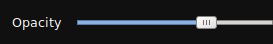
\includegraphics[height=1cm]{images/opacity-slider.png}
\caption{Trace opacity slider}
\label{opacityslider}
\end{figure}

\begin{figure}[H]
\centering
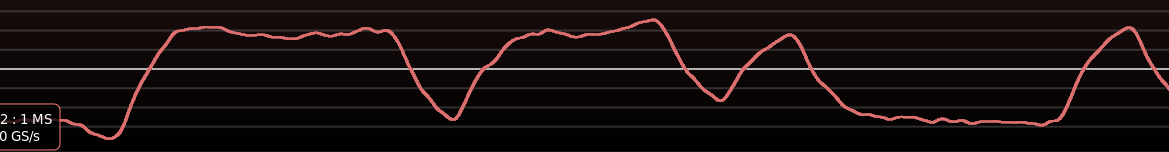
\includegraphics[width=10cm]{images/sparse-waveform.png}
\caption{Sparse waveform at a high zoom level}
\label{sparse-waveform}
\end{figure}

\begin{figure}[H]
\centering
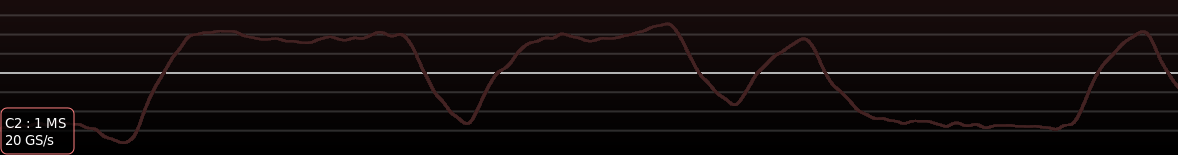
\includegraphics[width=10cm]{images/dim-waveform.png}
\caption{Dim waveform showing difficulty of seeing waveform at low opacity}
\label{dim-waveform}
\end{figure}

For example, the DVI waveform in Fig. \ref{washedout-waveform} looks like a solid white blob with a vaguely visible
outline. No fine detail can be observed other than the increased over/undershoot and random-looking edges on the
scanlines, compared to the flat appearance of the blanking period between scanlines and at the end of the frame.

When the opacity is reduced in this example, many more nuances of the signal become apparent. The high/low voltage
levels of the signal compared to the transitions between them are obvious, and the H/V sync pulses within the blanking
period show up as a slightly darker region.

\begin{figure}[H]
\centering
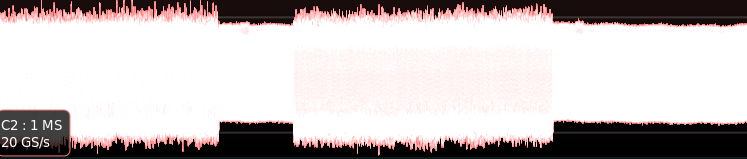
\includegraphics[width=10cm]{images/washedout-waveform.png}
\caption{Intensity-graded waveform showing washed-out appearance at high opacity}
\label{washedout-waveform}
\end{figure}

\begin{figure}[H]
\centering
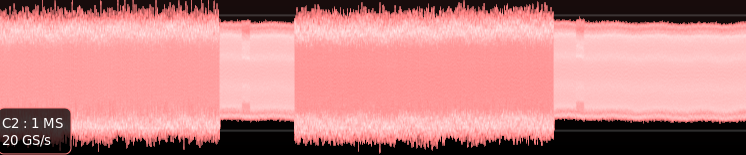
\includegraphics[width=10cm]{images/graded-waveform.png}
\caption{Intensity-graded waveform at lower opacity level}
\label{graded-waveform}
\end{figure}

As of this writing, the opacity setting is global for the entire application. Should this be changed to per waveform
group? If so, how should the group be selected and should there still be an option to make changes globally?
\end{comment}
